\scanpage{71}
\mspage{324}

\deleted{We must therefore \unsure{have}}

\unsure{Henceforth} we \unsure{restrict} ourselves to the automorphisms
(\inserted{\unsure{actual or}} outer) of $\widehat{\Pi}_{0,3}$
which \unsure{respect} the loop structure, and \unsure{commute} with
$\mathfrak S_3$ (as outer actions)
--- which \unsure{correspond} to the automorphisms
\inserted{(\unsure{actual or outer})} of
$\widehat{\mathfrak S}_{0,3}^{+}$ which \unsure{induce}
the identity on $\mathfrak S_3$,
and \unsure{satisfy} a) above. \deleted{They \illegible{1}}

The \uline{outer} \unsure{automorphisms} of this nature
\unsure{correspond} therefore to the actual automorphisms $u$
\inserted{of $\widehat{\Pi}_{0,3}$}
which \unsure{commute} with $\sigma_\infty$, i.e. $u$
\inserted{of $\widehat{\mathfrak S}_{0,3}^{+}$} which
\unsure{fix} $\sigma_\infty$, and are determined by a
$g\in\widehat{\Pi}_{0,3}$ satisfying (38), \uline{and} such that
in addition there exist \inserted{$p\in\widehat{\mathbb Z}^{*}$ and}
$g_0\in\widehat{\Pi}_{0,3}$ satisfying
\[
(39)\qquad
u(\ell'_0)=\operatorname{int}(g_0)({\ell'_0}^{p})
\qquad\text{i.e.}\qquad
u(\ell_0)=\operatorname{int}(g_0)(\ell_0^{p})
\]
(\unsure{where|i.e.} $g_0$ is determined modulo $L_0=\ell_0^{\widehat{\mathbb Z}}$
\unsure{\ldots}). Calculations made elsewhere \unsure{show}
\inserted{then} that we must have
\[
(40)\qquad g=\sigma_\infty(g_0)\,\ell_1^{\gamma}\,\rho(g_0)^{-1}
\]
\margin{with $\gamma\in\widehat{\mathbb Z}$ well determined
(\unsure{independent} of the choice of $g_0$)}
i.e.
\[
(41)\qquad
\deleted{\rho(g_0)}\,\sigma_\infty(g_0)^{-1}\,
\underbrace{g\rho(g_0)}_{\unsure{g_1}}\in L_1
=\unsure{\mathcal N|N|\mathrm{Norm}}_{\widehat{\Pi}_{0,3}}(L_1)
\]

\scanpage{72}

Indeed, we have by \unsure{hypothesis} on $g_0$ (cf. (39))
\[
(42)\qquad u(L_0)=\operatorname{int}(g_0)(L_0)
\]
\unsure{\deleted{hence}|hence}
\[
\begin{aligned}
&u\sigma_\infty(L_0)=u(L_1)\overset{40}{=}
  \operatorname{int}(g_1)(L_1)\\
&\Vert\quad(\text{since }u\sigma_\infty=\sigma_\infty u)\\
&\sigma_\infty u(L_0)\underset{(42)}{=}
 \sigma_\infty(\operatorname{int}(g_0)(L_0))
 =\operatorname{int}(\sigma_\infty(g_0))(\sigma_\infty(L_0))
 =\operatorname{int}(\sigma_\infty(g_0))(L_1)
\end{aligned}
\]
hence
\[
\operatorname{int}(\sigma_\infty(g_0)^{-1}g_1)(L_1)\subset L_1
\]
therefore
\[
\sigma_\infty(g_0)^{-1}\underbrace{g_1}_{g\rho(g_0)}
\in \mathcal N_{\widehat{\Pi}_{0,3}}(L_1)=L_1
\]
hence
\[
\sigma_\infty(g_0)^{-1}\unsure{g_1|g}\rho(g_0)=\ell_1^\gamma
\qquad (\gamma\in\widehat{\mathbb Z})
\]
hence (40). We will note, to \unsure{return to it}, that the element $g$
defined in terms of a $g_0$ \inserted{and of $\gamma$} \margin{$\checkmark$}
indeed depends only on $g_0$ modulo $L_0$. \deleted{\illegible{1}}

\margin{\figure{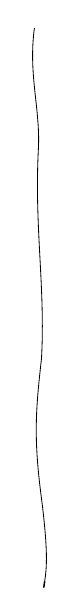
\begin{tikzpicture}[x=1cm,y=1cm,line cap=round]
\draw[line width=.30pt] (.03,0) .. controls (-.05,-.60) and (.11,-1.03) .. (.08,-1.55)
 .. controls (.03,-2.54) and (.17,-3.30) .. (.12,-4.20)
 .. controls (.04,-4.90) and (.02,-5.24) .. (.13,-6.05)
 .. controls (.20,-6.64) and (.19,-6.84) .. (.16,-7.03);
\draw[line width=.55pt] (.16,-7.03) -- (.15,-7.10);
\end{tikzpicture}}}
\unsure{Thus}; the datum of $u_0$
\deleted{\unsure{satisfying}} a loop \inserted{\unsure{outer automorphism}}
of $\widehat{\Pi}_{0,3}$ \unsure{commuting} with
$\mathfrak S_3$, or again
\unsure{an|$u$} outer automorphism of $\widehat{\mathfrak S}_{0,3}^{+}$
\unsure{inducing} the identity in $\mathfrak S_3$
and \deleted{\unsure{transforming}}
\inserted{\unsure{leaving invariant}} the conjugacy class
of the loop subgroup
$L'_0=\varepsilon_0^{\widehat{\mathbb Z}}={\ell'_0}^{\widehat{\mathbb Z}}
=\widehat{\varphi}(L_0)$,
or again that of a loop automorphism
$u_0$ of $\widehat{\Pi}_{0,3}$ \unsure{commuting} with
$\sigma_\infty$, and \unsure{in the outer automorphism quotien\textsuperscript{t}} with $\rho$,
or again of an automorphism $u$ of $\widehat{\mathfrak S}_{0,3}^{+}$
which fixes $\sigma_\infty$, and which fixes $\rho$ modulo $\widehat{\Pi}_{0,3}$
--- \unsure{is equivalent to} the datum of $g_0\in\widehat{\Pi}_{0,3}$ modulo $L_0$,
and of $\gamma\in\widehat{\mathbb Z}$, satisfying the relation

\scanpage{73}
\mspage{325}

\margin{\figure{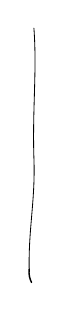
\begin{tikzpicture}[x=1cm,y=1cm,line cap=round]
\draw[line width=.30pt] (.04,0) .. controls (.08,-.55) and (.02,-1.02) .. (.04,-1.65)
 .. controls (.06,-2.18) and (-.03,-2.54) .. (-.02,-3.06);
\draw[line width=.52pt] (-.02,-3.06) .. controls (-.03,-3.13) and (-.01,-3.19) .. (.01,-3.23);
\end{tikzpicture}}}
\[
(38)\qquad \uline{g\rho(g)\rho^2(g)=1},
\]
where $g$ is given by (40), and where $u$ is expressed in terms of
\deleted{$g$} $g$ hence of $g_0,\gamma$ by
\[
(36)\qquad
\left\{\begin{aligned}
u(\sigma_\infty)&=\sigma_\infty\\
u(\rho)&=g\rho\qquad
\left(=\underbrace{\sigma_\infty(g_0)\ell_1^\gamma\rho(g_0)^{-1}}_g\rho\right).
\end{aligned}\right.
\]

\deleted{The relation (42)\inserted{\unsure{cf. = above}}, then reads,
since $L_0$ is generated by}
\[
\deleted{\ell_0=\underbrace{\ell'_0}_{\varepsilon_0}^{2}=(\sigma_\infty\rho)^2\deleted{\unsure{\sigma_\infty}}=\sigma_\infty\rho\sigma_\infty\rho}
\]
\[
\deleted{\underbrace{(u(\sigma_\infty\rho))}_{
\substack{\sigma_\infty g\rho=g_0\sigma_\infty \ell_1^\gamma\rho g_0^{-1}
=\operatorname{int}(g_0)(\sigma_\infty \ell_1^\gamma\rho)}}^{\unsure{2|4}}
\in\operatorname{int}(g_0)(\unsure{L'_0|L_0})\qquad\text{\unsure{now}}}
\]
\[
\deleted{\operatorname{int}(g_0)(\sigma_\infty \ell_1^\gamma\rho)^2\deleted{\unsure{g_0^{-1}}=1}}
\]
\deleted{thus (42) reads}
\[
\deleted{(\sigma_\infty \ell_1^\gamma\rho)^2\in L_0}
\]
\deleted{\unsure{i.e.}}
\[
\deleted{
\underbrace{\sigma_\infty \ell_1^\gamma\sigma_\infty}_{
    \underbrace{\sigma_\infty(\ell_1)}_{\ell_0}^{\gamma}}
  \underbrace{\sigma_\infty\illegible{1}\rho}_{\varepsilon_0}
}
\]
\margin{\deleted{N.B. $\operatorname{int}(g_0^{-1})u(\ell_0)$}}
\margin{\deleted{N.B. we have
$(\operatorname{int}(g_0^{-1})u)(\ell_0)
=(\sigma_\infty \ell_1^\gamma\rho)^2=\ell_0^{2\gamma+1}$}}
\deleted{\unsure{i.e.}}
\[
\deleted{\overset{\varepsilon_0^{2\gamma+1}}{\unsure{\ell_0^\gamma}\ \underbrace{\varepsilon_0}_{\unsure{\varepsilon_0^{2\gamma}}}}\in L_0}
\]
\deleted{therefore \unsure{\ldots}}
\[
\deleted{\unsure{\operatorname{int}(g_0)}\quad u(\ell_0)=}
\]

The relation (42), or the \unsure{apparently} stronger relation
\[
(43)\qquad u(L'_0)\subset\operatorname{int}(g_0)(L'_0)
\]
reads
\[
\underbrace{\operatorname{int}(g_0^{-1})\,
\underbrace{u(\underbrace{\sigma_\infty\rho}_{\ell'_0=\varepsilon_0})}_{
\sigma_\infty g\rho=g_0\sigma_\infty \ell_1^\gamma\rho g_0^{-1}}}_{
\sigma_\infty \ell_1^\gamma\rho
=\underbrace{\underbrace{\sigma_\infty \ell_1^\gamma\sigma_\infty}_{
 \underbrace{\sigma_\infty(\ell_1)^\gamma}_{\ell_0^\gamma=\varepsilon_0^{2\gamma}}}
\underbrace{\sigma_\infty\rho}_{\deleted{\unsure{\sigma_\infty\rho}}\varepsilon_0}}_{
\varepsilon_0^{2\gamma+1}}}
\in L'_0
\]
\margin{\uline{N.B.} we have
$\operatorname{int}(g_0^{-1})u(\underbrace{\ell'_0}_{\varepsilon_0})
=\varepsilon_0^{2\gamma+1}$}
\unsure{is satisfied} automatically, we \unsure{will have}
even
\[
\deleted{(44)\qquad u(\ell'_0)=u(\varepsilon_0)
=\operatorname{int}(g_0)(\ell'}
\]

\scanpage{74}

\[
(44)\qquad
u\bigl(\underset{\substack{\Vert\\ \varepsilon_0}}{\ell'_0}\bigr)
 = \operatorname{int}(g_0)\bigl(\underset{\substack{\Vert\\ \varepsilon_0}}{\ell'_0}{}^{p}\bigr)
\qquad \text{with}\quad \uuline{p=2\gamma+1}
\]
hence (39), \deleted{hence} on \unsure{raising} to the square:
\[
u(\ell_0)=\operatorname{int}(g_0)(\ell_0^p).
\]

\deleted{\unsure{We}}\quad
\uline{N.B.} We \unsure{will note} that if $p\in\widehat{\mathbb Z}^{*}$, then
$p-1\in 2\widehat{\mathbb Z}$ i.e.\ $\frac{p-1}{2}\in\widehat{\mathbb Z}$,
since it suffices to check the analogous relation for a $p\in\mathbb Z_\ell^{*}$,
\unsure{for|that} $p-1\in 2\mathbb Z_\ell$, now if $\ell\ne2$ we have
$2\mathbb Z_\ell=\mathbb Z_\ell$ OK, \unsure{there remains} the case $\ell=2$
$p\in\mathbb Z_2^{*}$ so the image of $p$ in $\mathbb Z/4\mathbb Z$
is $1$ or $3$ so $p-1\equiv0$ or $2\bmod4$
\deleted{\illegible{3}} so $\frac{p-1}{2}\in\mathbb Z_2$, OK.

\deleted{\unsure{It therefore remains to expri}}\par
It therefore remains to \unsure{express} condition (38), and we write it
\deleted{\unsure{in the form}}
\[
\underbrace{\sigma_\infty(g_0)\ell_1^\gamma\rho(g_0^{-1})}\,
\underbrace{\rho\sigma_\infty(g_0)\ell_\infty^\gamma\rho^2(g_0^{-1})}\,
\rho^2\sigma_\infty(g_0)\ell_0^\gamma g_0^{-1}=1
\]
i.e., on applying $\operatorname{int}(g_0^{-1})$ and
\deleted{\illegible{2}}\inserted{\unsure{setting again}}
(cf. (8))
\[
(45)\qquad g_0^{-1}\sigma_\infty(g_0)=h_0^{-1}
\qquad\text{i.e.}\quad
h_0=\sigma_\infty(g_0)^{-1}g_0=[\sigma_\infty,g_0^{-1}]
\]
\[
h_0^{-1}\ell_1^\gamma\underbrace{\rho(h_0^{-1})\ell_\infty^\gamma}\,
\rho^2(h_0^{-1})\ell_0^\gamma=1
\]
or again, on applying $\operatorname{int}(\ell_0^\gamma)$
\[
(46)\qquad
\boxed{\underbrace{(\ell_0^\gamma h_0^{-1})}\cdot
\rho(\ell_0^\gamma h_0^{-1})\cdot\rho^2(\ell_0^\gamma h_0^{-1})=1}
\qquad\left(\text{where }\gamma=\frac{p-1}{2}\right)
\]
which is none other than (10). As for the condition \unsure{(9)|(7)},
we see that it is \inserted{superfluous, i.e.,} automatically satisfied.